%%%%%%%%%%%%%%%%%%%%%%%%%%%%%%%%%%%%%%%%%
% a0poster Portrait Poster
% LaTeX Template
% Version 1.0 (22/06/13)
%
% The a0poster class was created by:
% Gerlinde Kettl and Matthias Weiser (tex@kettl.de)
% 
% This template has been downloaded from:
% http://www.LaTeXTemplates.com
%
% License:
% CC BY-NC-SA 3.0 (http://creativecommons.org/licenses/by-nc-sa/3.0/)
%
%%%%%%%%%%%%%%%%%%%%%%%%%%%%%%%%%%%%%%%%%

%----------------------------------------------------------------------------------------
%	PACKAGES AND OTHER DOCUMENT CONFIGURATIONS
%----------------------------------------------------------------------------------------

%\documentclass[a0,landscape,spa\documentclass[a0,landscape,spanish,20pt]{a0poster}nish,20pt]{a0poster}
\documentclass[a0,portrait,spanish,20pt]{a0poster}

\newcommand{\anchoFigura}{0.48}
\newcommand{\anchoFiguraPareto}{0.75}
% Include the helvet package
\usepackage{helvet}

% Set the default font to be palatino
\renewcommand{\sfdefault}{ppl}
%\usepackage[]{algorithm}
\usepackage{algpseudocode}
%S\usepackage[spanish, mexico]{babel}
%\selectlanguage{spanish}
\usepackage[utf8]{inputenc}
%\usepackage{float}
\usepackage{mathrsfs}
\usepackage{amsmath}
\usepackage{ragged2e}
\usepackage{multicol} % This is so we can have multiple columns of text side-by-side
\columnsep=100pt % This is the amount of white space between the columns in the poster
\columnseprule=3pt % This is the thickness of the black line between the columns in the poster
\usepackage{vwcol}  
\usepackage[svgnames]{xcolor} % Specify colors by their 'svgnames', for a full list of all colors available see here: http://www.latextemplates.com/svgnames-colors

%\usepackage{times} % Use the times font
\usepackage{palatino} % Uncomment to use the Palatino font

\usepackage{graphicx} % Required for including images
\graphicspath{{figures/}} % Location of the graphics files
\usepackage{booktabs} % Top and bottom rules for table
\usepackage[font=Large,labelfont=bf]{caption} % Required for specifying captions to tables and figures
\usepackage{amsfonts, amsmath, amsthm, amssymb} % For math fonts, symbols and environments
\usepackage{wrapfig} % Allows wrapping text around tables and figures

\usepackage{titlesec}
\usepackage{framed}
\usepackage[Large,bf, raggedright]{subfigure} % subfiguras
\usepackage{subfig}
\usepackage{floatrow}
\usepackage{pgfplots}
\usepackage{tabularx} % in the preamble
\usepackage[eulergreek]{sansmath}
\pgfplotsset{compat=1.3, width=70mm, height=60mm}
\pgfplotsset{
tick label style = {font=\sansmath\sffamily},
every axis label = {font=\sansmath\sffamily},
legend style = {font=\sansmath\sffamily},
label style = {font=\sansmath\sffamily}
}

\usepackage{esvect}
\usepackage{multirow}
\usetikzlibrary{spy}
\usetikzlibrary{arrows,shapes,positioning}
\usetikzlibrary{calc,decorations.markings}

\titlespacing*{\section}{0pt}{2pt}{0pt}
\definecolor{shadecolor}{rgb}{0.196078431,0.278431373,0.462745098}
\newcommand*{\bigH}{\scalebox{1.5}{\ensuremath{\mathscr{H}}}}

 % \usepackage[usenames,dvipsnames]{pstricks}
 % \usepackage{epsfig}
 % \usepackage{pst-grad} % For gradients
 % \usepackage{pst-plot} % For axes
 % \usepackage{auto-pst-pdf}
 % \usepackage{luatex85}
 \usepackage{standalone}
 \usepackage{caption}
\begin{document}

%----------------------------------------------------------------------------------------
%	POSTER HEADER 
%----------------------------------------------------------------------------------------

% The header is divided into two boxes:
% The first is 75% wide and houses the title, subtitle, names, university/organization and contact information
% The second is 25% wide and houses a logo for your university/organization or a photo of you
% The widths of these boxes can be easily edited to accommodate your content as you see fit
 
\begin{minipage}[b]{1\linewidth}
\begin{minipage}{0.60\linewidth}
\begin{shaded}
\centering
\Huge \color{White} \fontfamily{phv} \textbf{Mejora de Contraste de Imágenes a Color Usando un Framework de Optimización Multi-Objetivo
Framework}\\ [0.5cm]% Title
\Large \textbf{Luis G. Moré\textsuperscript{1}, Diego Pinto\textsuperscript{1}, José L. Vázquez\textsuperscript{1}} \\ 
\Large \textit{\textsuperscript{1}Facultad Politécnica - Universidad Nacional de Asunción}
\end{shaded}
\end{minipage}
\hspace*{1cm}
\begin{minipage}{0.15\linewidth}
\includegraphics[width=1\columnwidth]{figures/photo.jpg}
\end{minipage}
\hspace*{1cm}
\begin{minipage}{0.15\linewidth}
\centering
\includegraphics[width=1\columnwidth]{figures/LogoCTS-20.jpg}
\end{minipage}


\end{minipage}

\line(1,0){3100}

%
%\begin{minipage}[b]{0.25\linewidth}
%\includegraphics[width=19cm]{photo.jpg}\\
%\end{minipage}

%\vspace{0.5cm} % A bit of extra whitespace between the header and poster content

%----------------------------------------------------------------------------------------


\begin{multicols}{2} % This is how many columns your poster will be broken into, a portrait poster is generally split into 2 columns


%----------------------------------------------------------------------------------------
%   INTRODUCTION
%----------------------------------------------------------------------------------------

%\color{SaddleBrown} % SaddleBrown color for the introduction

\section*{ \begin{shaded} \color{White} \huge \centering Introducción \end{shaded}}



{ \Large 

\color{Black}

La Mejora del Contraste de Imágenes es una tarea importante debido a que pueden existir procesos posteriores que dependen fuertemente de él.

Aparecen nuevos problemas cuando se realiza CE de imágenes a color. Cuando se realiza CE de imágenes a color, se debe tener en cuenta la información de intensidad y la información de color (tal como los colores $R,G,B$). 

\textbf{Objective: }Obtener parámetros del Algoritmo de Mejora del Contraste cuya relación entre contraste y distorsión sea adecuada para obtener imágenes con distintos niveles de contraste. 

}

\color{Black} % DarkSlateGray color for the rest of the content

\section*{ \begin{shaded} \color{White} \huge \centering Método \end{shaded}}

{ \Large
\color{Black}

% \begin{figure}[H]
% %\vspace{-1pt}
% %\hspace{5pt}
% %\centering
% \includegraphics[{width=1\linewidth}]{figures/ccis2016.png}
% \caption{ \Large Interaction among $CLAHE$, $MOPSO$ particles and objective functions evaluation.}
% \label{fig:particula_clahe}
% \end{figure}


La Figura \ref{fig:particula_clahe} muestra cómo Color Many-Objective PSO-CLAHE ($CMOPSO-CLAHE$) basado en $SMPSO$ \cite{4938830} sintoniza los parámetros del algoritmo $CLAHE$ \cite{Zuiderveld:1994:CLA:180895.180940}. Durante el proceso los resultados candidatos se evalúan de acuerdo a las métricas  \textit{Entropía} ($\bigH_Y$)\cite{tsai2008information} y $SSIM$ \cite{wang2004image} para cada canal de color (denominados $SSIM_{R},SSIM_{G},SSIM_{B}$), y los mejores resultados conforman un Conjunto Pareto, que son los parámetros de $CLAHE$ que dan los mejores resultados en términos de proporción contraste/distorsión. 

}

\section*{ \begin{shaded} \color{White} \huge \centering Resultados \end{shaded}}

%----------------------------------------------------------------------------------------
%   MATERIALS AND METHODS
%----------------------------------------------------------------------------------------
\color{Black} % DarkSlateGray color for the rest of the content

{ \Large

\begin{itemize}

\item Se realizaron pruebas sobre 10 imágenes a color. Para cada imagen de prueba, se realizaron 50 ejecuciones de $CMOPSO-CLAHE$, con poblaciones compuestas por 100 partículas, y 100 iteraciones para cada ejecución. Aproximadamente 100-250 soluciones no dominadas se obtuvieron para cada imagen de prueba.
% \item The CE approach proposed in \cite{morepso} is adopted for comparison. Single-objective results are dominated when compared using many-objective evaluation function. This is clearly visible in Table \ref{table:nodominadas}.
% \item This is because the latter calculates $SSIM$ for every color channel $(R,G,B)$, meanwhile the single-objective approach only considers a weighted sum when optimizing images.
%\item The Pareto fronts for those images are shown in Figure \ref{fig:resultado_mammogram} and Figure \ref{fig:resultado_chest}.

\end{itemize}

}

% \begin{figure}[H]
% \centering
% \subfigure[]{\includegraphics[width=0.48\columnwidth]{figures/lena_color_512_lc.jpg}}
% \hspace{1pt}
% \subfigure[]{\includegraphics[width=0.48\columnwidth]{figures/0-resultado1.jpg}} \\[5pt]


% \caption{(a) Lenna Test Image. $SSIM$=1.0  \protect\bigH=6.91259 (b) Resultant image. (See Table \ref{tab:tabla1} for metric values)}
% \label{fig:resultado_chest}
% \end{figure}

% \begin{table}[H]
% \setlength{\abovecaptionskip}{2pt plus 3pt minus 2pt} % Chosen fairly arbitrarily
% \caption[Parámetros de entrada para $MOPSO$]{Metric coefficients obtained using our approach for some non-dominated results from image in Figure (\ref{fig:casa1}), and the coefficients obtained using the approach of \cite{morepso}.}
% \begin{center}
% \resizebox{0.9\columnwidth}{!}{%
%  \begin{tabular}{||c | c c c c||} 
%  \hline
%  & $\mathscr{H_Y}$ & $SSIM_R$ & $SSIM_G$ & $SSIM_B$ \\ 
% \hline
% Result 1 & 0.544854	& 0.0155038	 & 0.0140995  & 0.0149364 \\ 
% \hline
% Result 2& 0.658577	& 0.00551113 & 0.00494194 & 0.00529456 \\ 
% \hline
% Result 3& 0.0425715	& 0.394656	 & 0.380667	  & 0.39842 \\ 
% \hline
% Result 4& 0.0365424	& 0.401675	 & 0.388628	  & 0.402692 \\ 
% \hline
% Result 5& 0.0350595	& 0.416776	 & 0.403636	  & 0.417654 \\ 
% \hline
% Result 6& 0.611275	& 0.00897331 & 0.00823064 & 0.00851013 \\ 
% \hline
% Result 7& 0.0342894	& 0.420948	 & 0.408035	  & 0.421891 \\ 
% \hline
% Result Mono& 0.788927    & 0.000204143 & 0.0000526475 & 0.0000518143 \\
% \hline
% \end{tabular}
% }
% \end{center}
% \label{table:nodominadas}
% \end{table}

% \begin{table}[H]
% \begin{center}
%  \begin{tabular}{||c c c c c||} 
%  \hline
%  Name & $\bigH$ & $SSIM_R$ & $SSIM_G$ & $SSIM_B$ \\ [0.5ex] 
%  \hline\hline
%  lena\_many.jpg & 7.451087 & 0.879813 & 0.894753 & 0.894353 \\ 
%  \hline
%  lena\_mono.jpg & 3.52383 & 0.121137 & 0.130535 & 0.13814 \\
%  \hline
%  peppers\_many.jpg & 7.565911 & 0.860698 & 0.87937 & 0.87922 \\
%  \hline
%  peppers\_mono.jpg & 3.56565  & 0.127914 & 0.153184 & 0.15157 \\
%  \hline
% \end{tabular}
% \end{center}
% \caption{Comparison between images processed using single-objective and many-objective approaches.}
% \label{tab:tabla1}
% \end{table}


% \begin{figure}[H]

% \subfigure[]{\includegraphics[width=0.40\columnwidth]{figures/peppers_color_lc.jpg}}
% \hspace{1pt}
% \subfigure[]{\includegraphics[width=0.40\columnwidth]{figures/0-resultado2.jpg}}

% % \subfigure[]{

% % \pgfplotsset{every axis/.append style={
% % thick,
% % tick style={semithick}}}
% % \begin{tikzpicture}
% % \begin{axis}[height=12cm, width=0.95\columnwidth, xlabel={Entropy}, ylabel={SSIM},domain = 0:1, xtick={0.60,0.70,0.80,0.85,0.90,0.95,1.0},
% % ytick={0.0,0.2,0.4,0.6,0.8,1.0}]
% % \addplot+[
% % only marks,
% % scatter,
% % mark=halfcircle*,
% % mark size=2.9pt]
% % table[meta=label]
% % {scattered_chest.dat};
% % \addlegendentry{Pareto front};

% % \addplot+[
% % only marks,
% % scatter,
% % mark=oplus*,
% % colormap/greenyellow,
% % mark size=7pt]
% % coordinates{
% %     (0.6235,1)
% %     (0.8549,0.8032)
% %     (0.91393,0.6121)
% % };
% % \addlegendentry{Images (a),(b),(c)};


% % \end{axis}
% % \end{tikzpicture}

% % }
% %
% \caption{ (a) Peppers test image. $(SSIM_R,SSIM_G,SSIM_B)$=1.0, \protect\bigH=7.053228  (b) Resultant image. (See Table \ref{tab:tabla1} for metrics).}
% %\vspace{-1.1em}
% \end{figure}

\setcounter{subfigure}{0}
\begin{figure}[H]
    \centering
    \subfigure[][]{%[t]{0.45\textwidth}
        \includegraphics[width=0.47\columnwidth]{calhouse_0230.jpg}
        % \caption{Original Image. $\mathscr{H_Y}=0.207231$, $SSIM_R=1$, $SSIM_G=1$, $SSIM_B=1$}
        % \label{fig:casa1original}
    }
    \quad %add desired spacing between images, e. g. ~, \quad, \qquad, \hfill etc. 
      %(or a blank line to force the subfigure onto a new line)
    \subfigure[]{%[t]{0.45\textwidth}
        \includegraphics[width=0.47\columnwidth]{calhouse_0230_20-25165283474-10.jpg}
        % \caption{Enhanced Image. $\mathscr{H_Y}=0.611275$, $SSIM_R=0.00897331$, $SSIM_G=0.00823064$, $SSIM_B=0.00851013$}
        %\label{fig:casa1enhanced1}
    } \\
    \quad %add desired spacing between images, e. g. ~, \quad, \qquad, \hfill etc. 
    %(or a blank line to force the subfigure onto a new line)
    \subfigure[]{%[t]{0.45\textwidth}
        \includegraphics[width=0.47\columnwidth]{calhouse_0230_20-62968204656-00.jpg}
        % \caption{Enhanced Image.  $\mathscr{H_Y}=0.0350595$, $SSIM_R=0.416776$, $SSIM_G=0.403636$, $SSIM_B=0.417654$}
        %\label{fig:casa1enhanced2}
    } 
    \subfigure[]{%[t]{0.45\textwidth}
        \includegraphics[width=0.47\columnwidth]{calhouse_0230_20-20-0020072469292179818.jpg}
        % \caption{Enhanced Image using \cite{morepso}. $\mathscr{H_Y}=0.788927$, $SSIM_R=0.000204143$, $SSIM_G=0.0000526475$, $SSIM_B=0.0000518143$}
        % \label{fig:casa1enhanced3}
    }

    \caption{Resultados Visuales. (a) Imagen Original. (b),(c),(d) Imágenes resultantes obtenidas a partir de $CMPOSO-CLAHE$\label{fig:casa1}}
\end{figure}

% \begin{table}[H]
% \setlength{\abovecaptionskip}{2pt plus 3pt minus 2pt} % Chosen fairly arbitrarily
% \caption[Parámetros de entrada para $MOPSO$]{Correlation table between metrics. Data was taken from Table \ref{table:nodominadas}. The strong negative correlation between $\mathscr{H_Y}$ and $SSIM_R$, $SSIM_G$, $SSIM_B$ indicates that a Bi-Objective approach might be suitable.}
% \begin{center}
% \resizebox{0.6\columnwidth}{!}{%
%  \begin{tabular}{||c | c c c c||} 
%  \hline
% Metrics & $\mathscr{H_Y}$ & $SSIM_R$ & $SSIM_G$ & $SSIM_B$ \\ 
% \hline
% $\mathscr{H_Y}$ & 1 &   &   &  \\ 
% \hline
% $SSIM_R$ & -0.9826  & 1 &  &  \\ 
% \hline
% $SSIM_G$ & -0.9823 & 0.9999   & 1   &  \\ 
% \hline
% $SSIM_B$ & -0.9826 & 0.9999   & 0.9999   & 1 \\ 
% \hline
% \end{tabular}
% }
% \end{center}
% \label{table:correlacion}
% \end{table}

%------------------------------------------------


\color{DarkSlateGray} % Set the color back to DarkSlateGray for the rest of the content


\section*{\vspace{-2em} \begin{shaded} \color{White} \huge \centering Conclusions \end{shaded}}

{
\Large
\justifying
$CMOPSO-CLAHE$ es una propuesta satisfactoria para la realización de la Mejora del Contraste Automática.

Como trabajos futuros, sería deseable experimentar la propuesta y medirla contra implementaciones parecidas del estado del arte, además de buscar mejoras en la eficiencia en los algoritmos de Mejora de Contraste Basado en Metaheurísticas.
%\item \textbf{Future work:} Test optimization-based contrast enhancement using new metaheuristics, IQA metrics, and public image databases. Establish new compromises between metrics, analytically and using Pareto fronts.
 

\small
\bibliography{refs}
\bibliographystyle{ieeetr}

}

%\section*{\begin{shaded} \color{White} \huge \centering Acknowledgments and info \end{shaded}}
%\centering
%\frame{\includegraphics[width=0.21\columnwidth]{figures/photo.jpg}}
%\hspace{1pt}
%\frame{\includegraphics[width=0.21\columnwidth]{figures/qrcode.jpg}}

%----------------------------------------------------------------------------------------
%	CONCLUSIONS
%----------------------------------------------------------------------------------------

\end{multicols}

\begin{figure}[H]
\centering
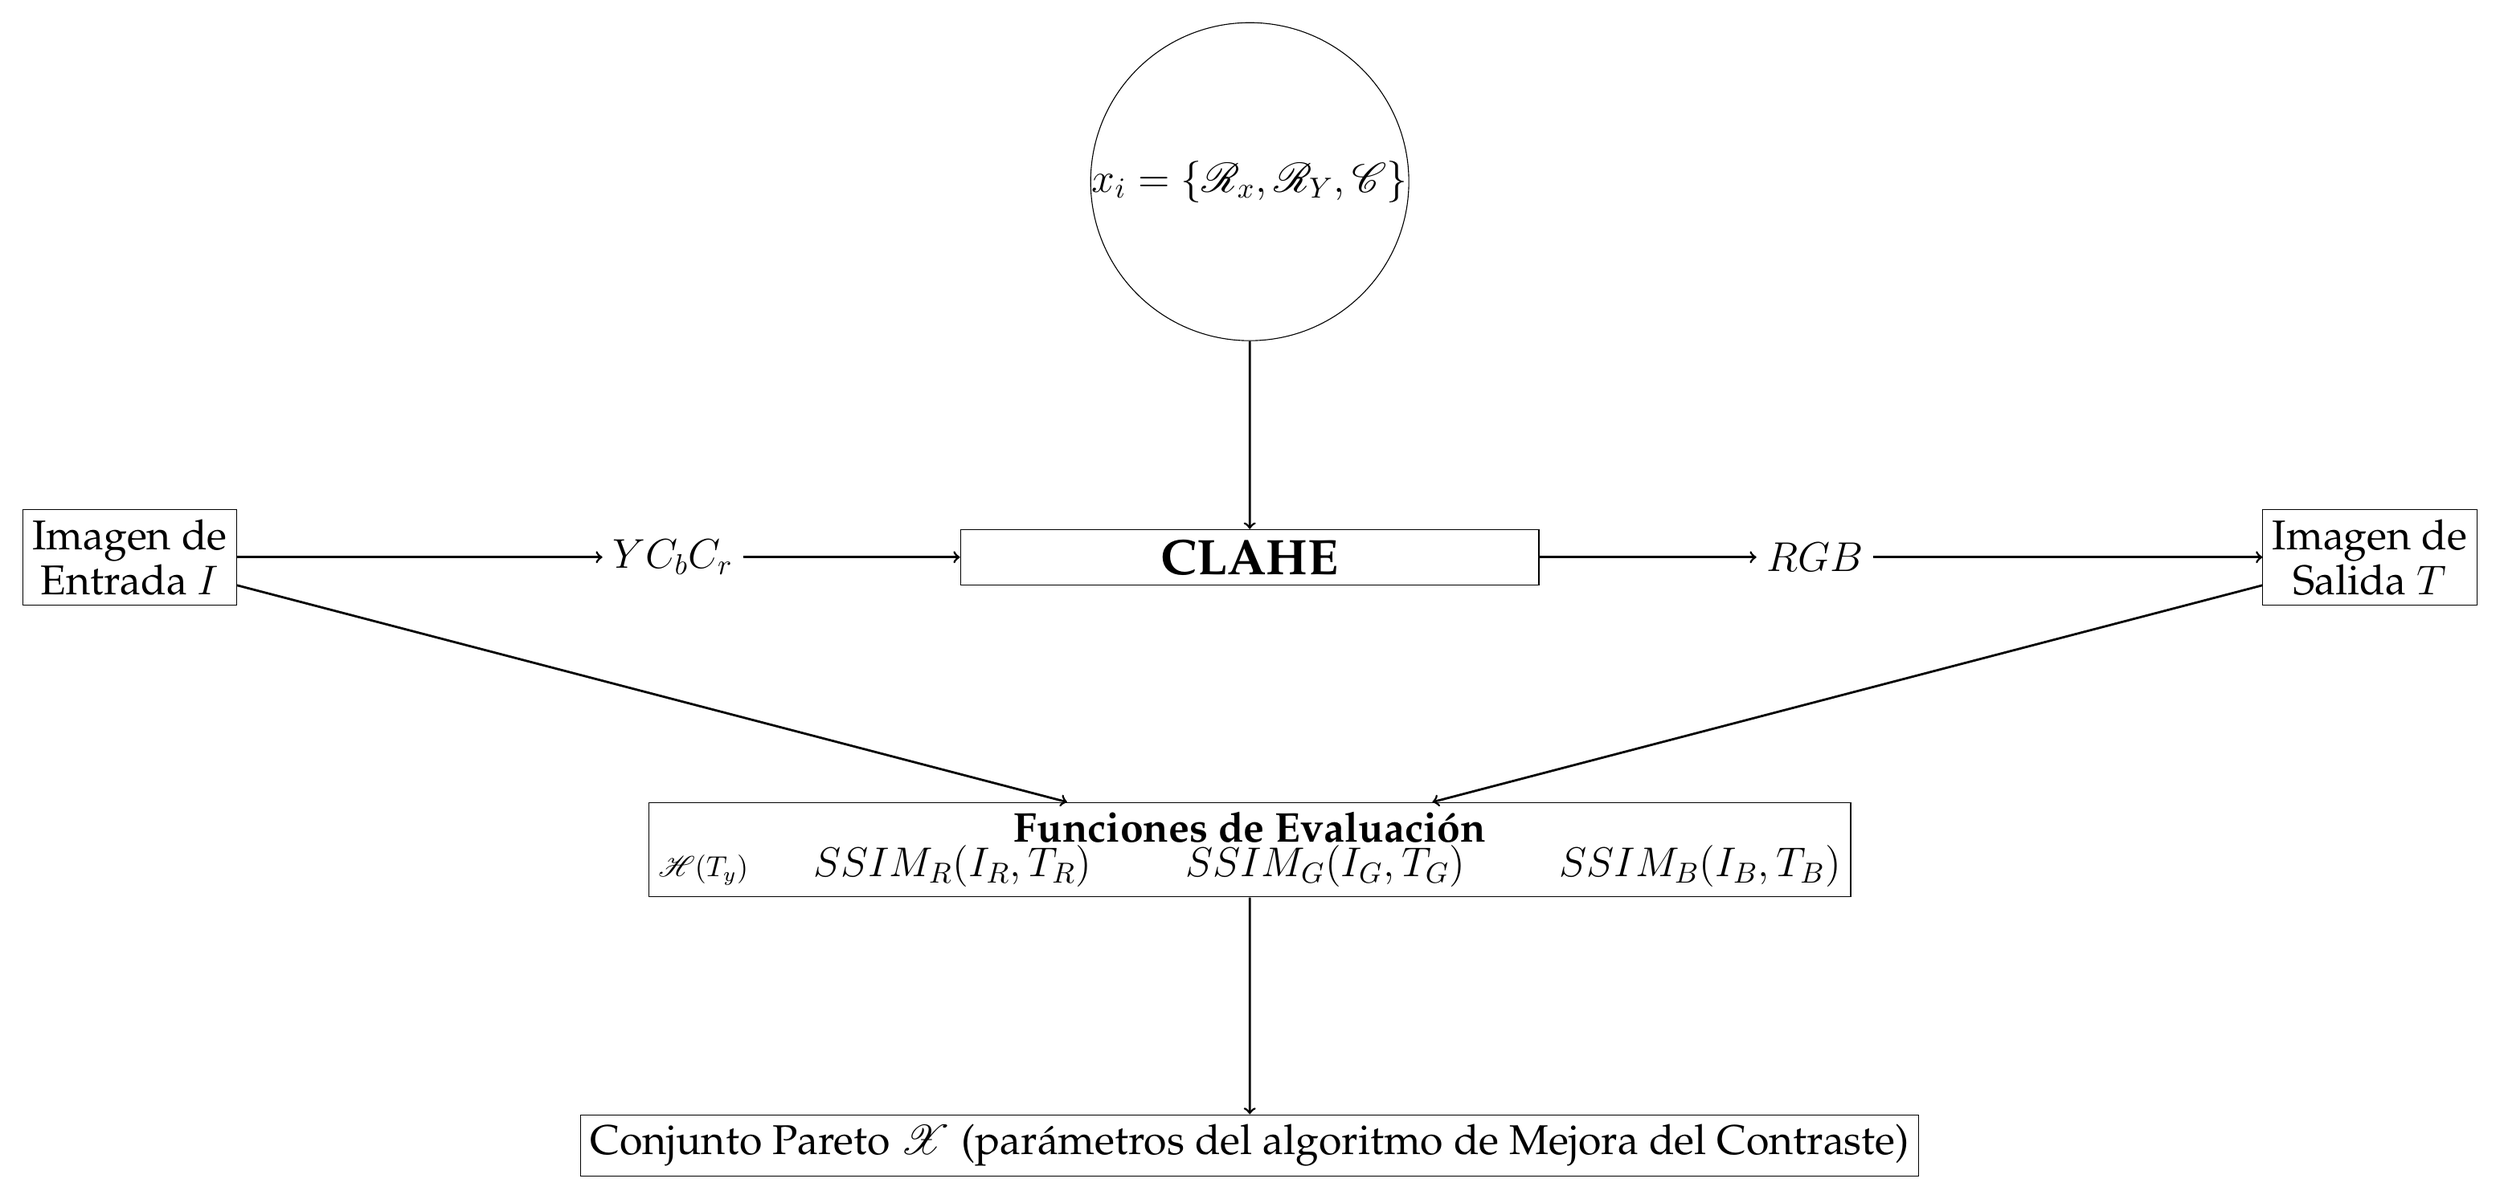
\begin{tikzpicture}[scale=1.3, transform shape]

%textos

%\node[draw,align=center] at (3,4) {\textbf{MANY-PSO-CLAHE}};
                                   
\node[draw,align=center,minimum width=200pt] (manypsoclahe) {\LARGE \textbf{CLAHE}};

\node[draw,align=center,below= 75pt of manypsoclahe] (evaluationfunctions) {\Large \textbf{Funciones de Evaluación}\\ $\mathscr{H}(T_y)$ \qquad \Large $SSIM_R(I_R,T_R)$ \qquad $SSIM_G(I_G,T_G)$ \qquad $SSIM_B(I_B,T_B)$};
                                   
\node[draw,align=center,below= 75pt of evaluationfunctions] (paretoset) {\Large Conjunto Pareto $\mathscr{X}$ (parámetros del algoritmo de Mejora del Contraste)};

\node[draw,align=center,left= 250pt of manypsoclahe] (inputimage) {\Large Imagen de \\ \Large Entrada $I$};

\node[draw,align=center,right= 250pt of manypsoclahe] (outputimage) {\Large Imagen de \\ \Large Salida $T$};

% \node[draw,circle,minimum size=1cm,inner sep=0pt,above left= 65pt and -40pt of manypsoclahe] (partic1) {\small $\mathscr{R}_x,\mathscr{R}_Y,\mathscr{C}$};

\node[draw,circle,minimum size=1cm,inner sep=0pt,above = 65pt of manypsoclahe] (partic2) {\Large $\vv{x_i}=\{\mathscr{R}_x,\mathscr{R}_Y,\mathscr{C}\}$};

% \node[draw,circle,minimum size=1cm,inner sep=0pt,above right= 65pt and -40pt of manypsoclahe] (partic3) {\small $\mathscr{R}_x,\mathscr{R}_Y,\mathscr{C}$};

\node[align=center,left= 75pt of manypsoclahe] (ycrcb) {\Large $YC_bC_r$};

\node[align=center,right= 75pt of manypsoclahe] (rgb) {\Large $RGB$};

\draw[->,draw=black,line width=1pt]
  % (partic1) edge (manypsoclahe) 
  (partic2) edge (manypsoclahe)
  % (partic3) edge (manypsoclahe)
  (inputimage) edge (ycrcb)
  (ycrcb) edge (manypsoclahe)
  (manypsoclahe) edge (rgb)
  (rgb) edge (outputimage)
  (outputimage) edge (evaluationfunctions)
  (inputimage) edge (evaluationfunctions)
  (evaluationfunctions) edge (paretoset);

\end{tikzpicture}
\caption{Proceso de evaluación de una solución potencial, para una iteración $t$ de la implementación.}
\label{fig:particula_clahe}
\end{figure}

\end{document}